\documentclass[DIV=calc, paper=a4, fontsize=11pt]{scrartcl}


\usepackage{makeidx}
\usepackage{graphicx}
\usepackage{flushend}

\usepackage{lmodern}
\usepackage[left=1.5cm,right=1.5cm,top=2.5cm,bottom=2cm]{geometry}
\usepackage{float}		
\bibliographystyle{plain} 
\pagestyle{plain} 
\pagenumbering{arabic}
\usepackage{fancyhdr} 	


\usepackage[T1]{fontenc}
\usepackage[utf8]{inputenc}
\usepackage[spanish]{babel}
\usepackage{hyperref}
\usepackage{graphicx}

\usepackage{lipsum}
\usepackage[protrusion=true,expansion=true]{microtype}
\usepackage{amsmath,amsfonts,amsthm}
\usepackage[svgnames]{xcolor}
\usepackage[svgnames]{xcolor}
\usepackage{booktabs}
\usepackage{fix-cm}
\usepackage{multicol}
\usepackage{siunitx}
\newenvironment{Figura}
  {\par\medskip\noindent\minipage{\linewidth}}
  {\endminipage\par\medskip}

\usepackage{sectsty}
\allsectionsfont{\usefont{OT1}{phv}{b}{n}}

\usepackage{fancyhdr}
\pagestyle{fancy}
\usepackage{lastpage}

\lhead{}
\chead{}
\rhead{}

\lfoot{}
\cfoot{}
\rfoot{\footnotesize Page \thepage\ of \pageref{LastPage}}

\renewcommand{\headrulewidth}{0.0pt}
\renewcommand{\footrulewidth}{0.4pt}

\usepackage{lettrine}
\newcommand{\initial}[1]{\lettrine[lines=3,lhang=0.3,nindent=0em]{
\color{DarkGoldenrod}{\textsf{#1}}}{}}

\usepackage{titling}

\newcommand{\HorRule}{\color{DarkGoldenrod} \rule{\linewidth}{1pt}}

\pretitle{\vspace{-120pt} \begin{flushleft} \HorRule \fontsize{22}{35} \usefont{OT1}{phv}{b}{n} \color{DarkRed} \selectfont}

\title{Coeficiente de Dilatación Térmica\\ %Aquí va el nombre de la práctica 
Práctica 6} %Numero de la práctica 

\posttitle{\par\end{flushleft}\vskip 0.5em}

\preauthor{\begin{flushleft}\large \lineskip 0.5em \usefont{OT1}{phv}{b}{sl} \color{DarkRed}}

\author{Misael Iván Macías Márquez\\
misaelmacias@ciencias.unam.mx}

\postauthor{\footnotesize \usefont{OT1}{phv}{m}{sl} \color{Black}

\vspace*{0.1cm} Facultad de Ciencias, UNAM

\par\end{flushleft}\HorRule}

\date{1 de Mayo de 2022\\Semestre 2022-2}


\begin{document}

\maketitle


\begin{abstract}
\textbf{Resumen:} Se determino el coeficiente de dilatación térmico lineal para el cobre, hierro y aluminio usando datos recabados experimentalmente por 2 grupos de alumnos, Los coeficientes de dilatación térmicos para el cobre, hierro y aluminio obtenidos son $(32.2 \pm 13) \times 10^{6}\frac{1}{^{\circ}C}$, $(47 \pm 15) \times 10^{6} \frac{1}{^{\circ}C}$ y $(16.3 \pm 4) \times 10^{6} \frac{1}{^{\circ}C}$ respectivamente, con discrepancias de $0.09$, $0.15$ y $1.78$ veces sus incertidumbres absolutas.
\end{abstract}

\begin{multicols}{2}




\section*{Introducción}

Cuando aumenta la temperatura, los átomos vibran con una amplitud mayor, y la distancia promedio entre los átomos aumenta. (Véase el estudio de la base microscópica de la dilatación térmica al final de esta sección.) Esto conduce a una dilatación de todo el cuerpo sólido. El cambio en cualquier dimensión lineal del sólido, tal como su longitud, su ancho, o su espesor, se llama dilatación lineal. Si la longitud de esta dimensión lineal es $L$, el cambio de temperatura $\Delta T$ causa un cambio de longitud $\Delta L$. Por medio de la experimentación hallamos que, si $\Delta T$ es lo suficientemente pequeña, este cambio de longitud $\Delta L$ es proporcional al cambio de temperatura $\Delta T$ y a la longitud original $L$. Por lo tanto, podemos escribir[1]


\begin{equation}
    \Delta L = \alpha (L \Delta T)
\end{equation}

donde $\alpha$ es el coeficiente de dilatación lineal[1].


\section*{Desarrollo experimental}

\begin{Figura}
\centering
    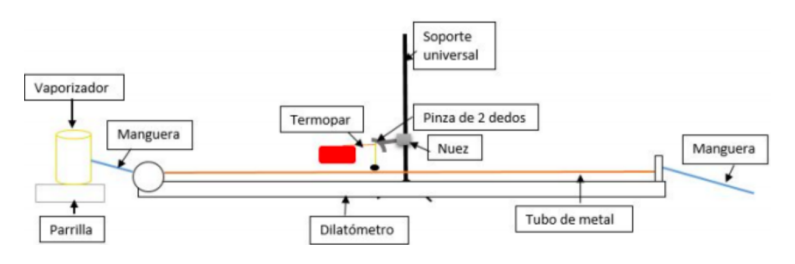
\includegraphics[width=1.1\textwidth]{diagrama dilatacion.PNG}
    \captionof{figure}{Diagrama del montaje experimental.}
    \label{fig}
\end{Figura}

\begin{Figura}
\centering
    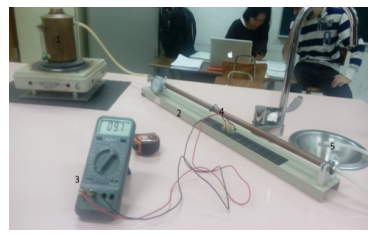
\includegraphics[width=0.8\textwidth]{dilatacion 1.PNG}
    \captionof{figure}{Material y arreglo experimental:  (1) generador de vapor, (2) dilatómetro, (3)multímetro, (4) termistor y (5) manguera. Montaje para el caso
de que el dilatómetro tenga termistor}
    \label{fig}
\end{Figura}

La práctica fue realizada por otro grupo de estudiantes, su desarrollo experimental es el siguiente:

\begin{enumerate}
    \item Con ayuda del flexómetro medir la longitud inicial de las varillas.
    
    \item Conectar el dilatómetro con termistor con ayuda de la manguera al generador de vapor.
    
    \item En el otro extremo del dilatómetro se conecta una manguera para que por ella salga el vapor que entra del debido al generador, figura (1).
    
    \item Llenar generador de vapor con agua hasta 3/4 partes de su capacidad.
    
    \item Colocar el generador de vapor sobre la parrilla y calentarlo.
    
    \item . Pegar la varilla al termistor del dilatómetro con ayuda de la tuerca.
    
    \item Conectar los cables banana banana del dilatómetro al multímetro.
    
    \item Ajustar el multímetro en $K\Omega$ para posteriormente hacer la conversión a $^{\circ}C$ para poder conocer la temperatura de cada varilla, figura (2).
    
    \item Una vez generado el vapor, este pasara a través de la manguera hacia la varilla (lo cual provocara que se comience a dilatar). Usando el dilatómetro medir la longitud de dilatación a cada $\Delta T$.

\end{enumerate}
    


\section*{Resultados y Análisis}

\subsection*{Cobre}

\begin{Figura}
\centering
    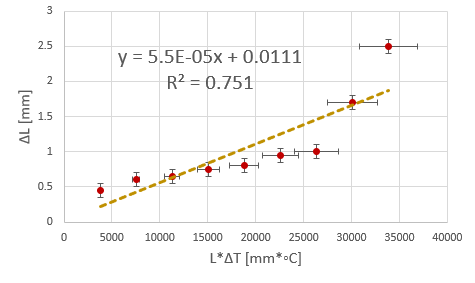
\includegraphics[width=0.8\textwidth]{grafica/cobreA.PNG}
    \captionof{figure}{Gráfica de ecuación 1 linealizada y ajustada para el cobre del grupo A.}
    \label{fig}
\end{Figura}

El grupo A nos da un coeficiente de dilatación lineal para el cobre de:

\begin{equation*}
    \alpha_{c} = (55 \pm 12)\times 10^{6} \frac{1}{^{\circ}C}
\end{equation*}


\begin{Figura}
\centering
    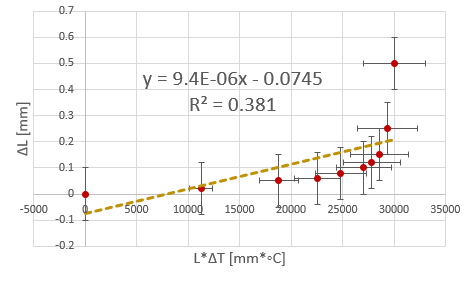
\includegraphics[width=0.8\textwidth]{grafica/cobreB.PNG}
    \captionof{figure}{Gráfica de ecuación 1 linealizada y ajustada para el cobre del grupo B.}
    \label{fig}
\end{Figura}

El grupo B nos da un coeficiente de dilatación lineal para el cobre de:

\begin{equation*}
    \alpha_{c} = (9.4 \pm 4.2)\times 10^{6} \frac{1}{^{\circ}C}
\end{equation*}


Promediando los resultados de ambos grupos y sumando por cuadraturas sus incertidumbres, nos da un resultado final de:

\begin{equation*}
    \alpha_{c} = (32.2 \pm 13)\times 10^{6} \frac{1}{^{\circ}C}
\end{equation*}

El coeficiente de dilatación lineal para el cobre reportado en la literatura es $33.4 \times 10^{6} \frac{1}{^{\circ}C}$.

\subsection*{Aluminio}

\begin{Figura}
\centering
    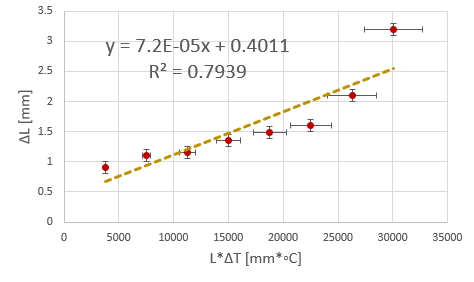
\includegraphics[width=0.8\textwidth]{grafica/aluminioA.PNG}
    \captionof{figure}{Gráfica de ecuación 1 linealizada y ajustada para el aluminio del grupo A.}
    \label{fig}
\end{Figura}

El grupo A nos da un coeficiente de dilatación lineal para el aluminio de:

\begin{equation*}
    \alpha_{a} = (72 \pm 15) \times 10^{6} \frac{1}{^{\circ}C}
\end{equation*}

\begin{Figura}
\centering
    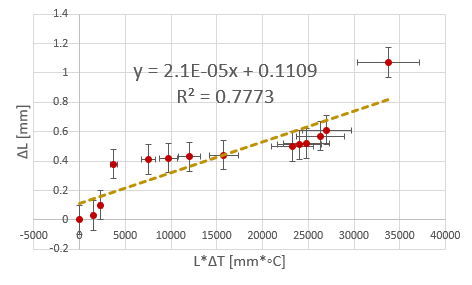
\includegraphics[width=0.8\textwidth]{grafica/aluminioB.PNG}
    \captionof{figure}{Gráfica de ecuación 1 linealizada y ajustada para el aluminio del grupo B.}
    \label{fig}
\end{Figura}

El grupo B nos da un coeficiente de dilatación lineal para el aluminio de:

\begin{equation*}
    \alpha_{a} = (21 \pm 3) \times 10^{6} \frac{1}{^{\circ}C}
\end{equation*}

Promediando los resultados de ambos grupos y sumando por cuadraturas sus incertidumbres, nos da un resultado final de:

\begin{equation*}
    \alpha_{a} = (47 \pm 15 ) \times 10^{6} \frac{1}{^{\circ}C}
\end{equation*}

El coeficiente de dilatación lineal para el aluminio reportado en la literatura es $44.8 \times 10^{6} \frac{1}{^{\circ}C}$.

\subsection*{Hierro}

\begin{Figura}
\centering
    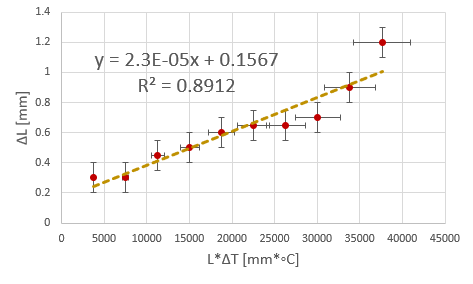
\includegraphics[width=0.8\textwidth]{grafica/hierroA.PNG}
    \captionof{figure}{Gráfica de ecuación 1 linealizada y ajustada para el hierro del grupo A.}
    \label{fig}
\end{Figura}

EL grupo A nos da un coeficiente de dilatación lineal para el hierro de:

\begin{equation*}
    \alpha_{h} = (23 \pm 3) \times 10^{6} \frac{1}{^{\circ}C}
\end{equation*}

\begin{Figura}
\centering
    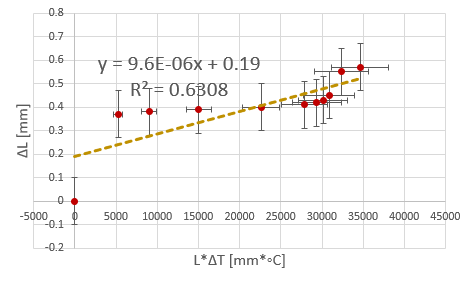
\includegraphics[width=0.8\textwidth]{grafica/hierroB.PNG}
    \captionof{figure}{Gráfica de ecuación 1 linealizada y ajustada para el hierro del grupo B.}
    \label{fig}
\end{Figura}

El grupo B nos da un coeficiente de dilatación lineal para el hierro de:

\begin{equation*}
    \alpha_{h} = (9.6 \pm 2.5)  \times 10^{6} \frac{1}{^{\circ}C}
\end{equation*}

Promediando los resultados de ambos grupos y sumando por cuadraturas sus incertidumbres, nos da un resultado final de:

\begin{equation*}
    \alpha_{h} = (16.3 \pm 4) \times 10^{6} \frac{1}{^{\circ}C}
\end{equation*}

El coeficiente de dilatación lineal para el hierro reportado en la literatura es $23.4 \times 10^{6} \frac{1}{^{\circ}C}$.


\section*{Conclusiones}

Los coeficientes de dilatación obtenidos para el grupo A y grupo B no fueron exactos pero al promediar los mismos estos errores se compensaron y los coeficientes de dilatación correspondieron de mejor manera a los reportados en la literatura. Las discrepancias para cada coeficiente de dilatación obtenidos son $0.09$, $0.15$ y $1.78$ veces sus incertidumbres absolutas para el cobre. aluminio y hierro respectivamente, que al ser menores a $2$ se pueden considerar resultados satisfactorios.
  
\begin{thebibliography}{99}
\bibitem{1} Resnick, R., Halliday, D., & Krane, K. (2002a). Física. Vol. 1( 5ta Edición) (5.a ed.). Grupo Editorial Patria.

\bibitem{1} https://moodle.fciencias.unam.mx/cursos/pluginfile.php/

151806/mod$_$resource/content/1/P6\%20Coeficiente

\%20de\%20dilataci\%C3\%B3n.pdf

\end{thebibliography}

\section*{Apéndices}

\subsection*{Tablas}

\begin{Figura}
\centering
    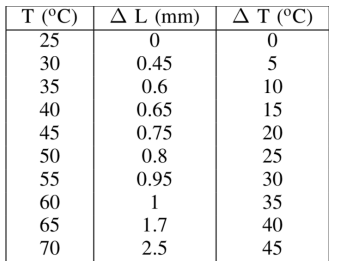
\includegraphics[width=0.8\textwidth]{tablas/tabla 1.PNG}
    \captionof{table}{Medidas obtenidas para la barra de cobre.}
    \label{fig}
\end{Figura}

\begin{Figura}
\centering
    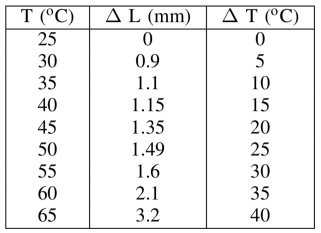
\includegraphics[width=0.8\textwidth]{tablas/tabla 2.PNG}
    \captionof{table}{Medidas obtenidas para la barra de aluminio.}
    \label{fig}
\end{Figura}

\begin{Figura}
\centering
    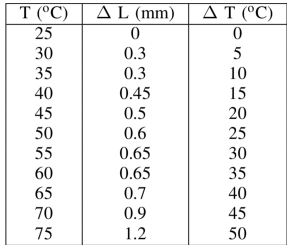
\includegraphics[width=0.8\textwidth]{tablas/tabla 3.PNG}
    \captionof{table}{Medidas obtenidas para la barra de hierro.}
    \label{fig}
\end{Figura}

\begin{Figura}
\centering
    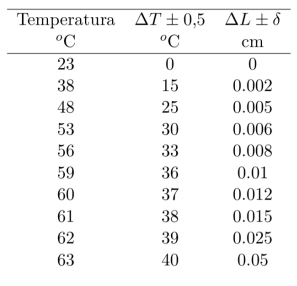
\includegraphics[width=0.8\textwidth]{tablas/tabla 4.PNG}
    \captionof{table}{Medidas obtenidas para la barra de cobre.}
    \label{fig}
\end{Figura}

\begin{Figura}
\centering
    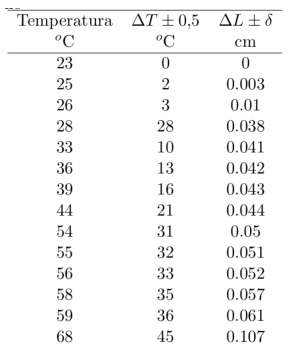
\includegraphics[width=0.8\textwidth]{tablas/tabla 5.PNG}
    \captionof{table}{Medidas obtenidas para la barra de aluminio.}
    \label{fig}
\end{Figura}

\begin{Figura}
\centering
    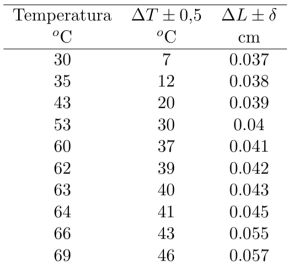
\includegraphics[width=0.8\textwidth]{tablas/tabla 6.PNG}
    \captionof{table}{Medidas obtenidas para la barra de hierro.}
    \label{fig}
\end{Figura}


\end{multicols}

\newpage

\subsection*{Dilatómetro}


Es un instrumento que sirve para medir el alargamiento que experimenta un cuerpo al incrementar la temperatura. La medición ayuda a encontrar el coeficiente de contracción o dilatación de un material en particular, a diferentes temperaturas. 

$\\$

\begin{figure}
    \centering
    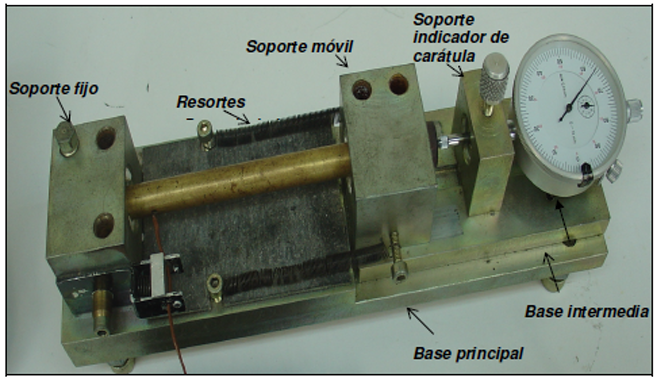
\includegraphics{dilatometro.PNG}
    \caption{Caption}
    \label{fig:my_label}
\end{figure}

\textbf{Base principal}: Su función es servir de base a los soportes fijo, móvil y soporte indicador de carátula, así como también de la base intermedia. Se encuentra soportada en cuatro tornillos.

$\\$

\textbf{Base intermedia}: Su función es sostener el soporte del indicador de carátula y el soporte móvil. La base intermedia va atornillada a la base principal, además tiene un canal por donde se desliza el soporte móvil.

$\\$

\textbf{Soporte fijo}: Su función es servir de soporte a la probeta cuando se va a realizar la medición.  Para evitar la transferencia de 7   Laboratorio de Producción. calor por parte de la probeta en el soporte,  se aloja una cerámica cilíndrica que está adherida en su interior.

$\\$

\textbf{Soporte móvil}:  Al igual que el soporte fijo, este evita la transferencia de calor mediante una cerámica adherida con un adhesivo refractario dentro del soporte, la cual sirve de apoyo a la probeta.   A los lados se encuentran un par de tornillos los cuales reciben los resortes que le ayudan a dar empuje para registrar la medición.

$\\$

\textbf{Soporte indicador de carátula}: Su función es alojar el indicador de carátula para registrar la medición de la contracción del material.

$\\$

\textbf{Indicador de carátula}:Instrumento utilizado para medir la contracción longitudinal de la probeta a medida que se enfría. Está dividida en centésimas de milímetro. Este aparato tiene dos relojes; el exterior es el que indica la contracción de la longitud, y el interior, es el que indica la cantidad de vueltas que da el reloj exterior. Cada división del reloj interior (1 mm) corresponde a 100 divisiones del reloj exterior. 

$\\$

\textbf{Probeta}:Son tubos o barras sólidas con los cuales hacemos las prácticas del laboratorio del dilatómetro. 




\end{document}